\chapter{Numerical Results in the Time-Driven Approach}
This chapter is dedicated to presenting the results obtained by applying the Stochastic Reachability approach (discussed in Chapter \ref{chpt:Model_Description}) to asset allocation. We recall that the output of the ODAA algorithm (see Theorem (\ref{thm:rec_algo})) is a sequence of allocation maps $\pi^{\star}=\{\mu_0^{\star},\ldots,\mu_{N-1}^{\star}\}$. For any portfolio realization $x \in \mathbb{R}$ at time $k \in \mathbb{N}$, the maps $\mu_k^{\star}$ provides us with the optimal asset allocation $\mu_k^{\star}(x)=\bm{u}_k^{\star}$; for instance, if $\bm{u}_k^{\star}= \begin{bmatrix}
0.2 & 0.2 & 0.6
\end{bmatrix}^T$ this means that 20\% of investor's wealth should be allocated to the first asset class, 20\% to the second one and the remaining 60\% to the third one. Objective of this chapter is to see what form these maps have at different time instant. The chapter unfolds as follows: in Section \ref{sec:The_Dataset} the dataset is presented and summarized by some sample statistics, in Section \ref{sec:Allocation_Maps} the parameters of the asset allocation problems are set and the allocation maps for the different models discussed in Chapter \ref{chpt:assetclass_returns} are reported.

\section{The Dataset}\label{sec:The_Dataset}
Our asset class menu consists of cash, bond and equity. To represent these markets we adopt the indexes presented in Table \ref{tab:indexes}.
\begin{table}[h] \label{tab:indexes}
	\centering
	\begin{tabular}{@{}lll@{}} \toprule
		Label & Asset Class & Index\\ \midrule
		C & Money Market & iShares Short Treasury Bond ETF\\
		\addlinespace[0.5em]
		B & US Bond  & Northern US Treasury Index \\
		\addlinespace[0.5em]
	    E &	US Equity &  {S\&P 500}\\ \bottomrule
		\addlinespace[0.5em]
	\end{tabular}
	\caption{Asset class and relative index}
\end{table}
The dataset is composed of weekly time series from 23 January 2010 to 15 April 2016. Data is downloaded from Yahoo Finance which is also where the reader is referred for more details of index composition. Asset class statistical indicators are summarized in Figure \ref{fig:assetclassReturns} and Table \ref{tab:sampleStatistics}. By comparing the annualized Mean return, it is clear that asset class Equity leads to higher performance than Bond and Bond, in turn, ensures higher performance than Cash. The annualized volatility tells us that the same hierarchy holds true also in terms of riskiness, being Equity the riskiest investment and Cash the least. Higher sample moments (Skewness and Kurtosis) suggest that the multivariate return distribution diverges significantly from a Gaussian one. Indeed, a quantitaive proof of this fact is given us from the Henze-Zirkler multivariate normality test which exhibits a zero p-value. 
\begin{figure}[h]\label{fig:assetclassReturns}
	\centering
	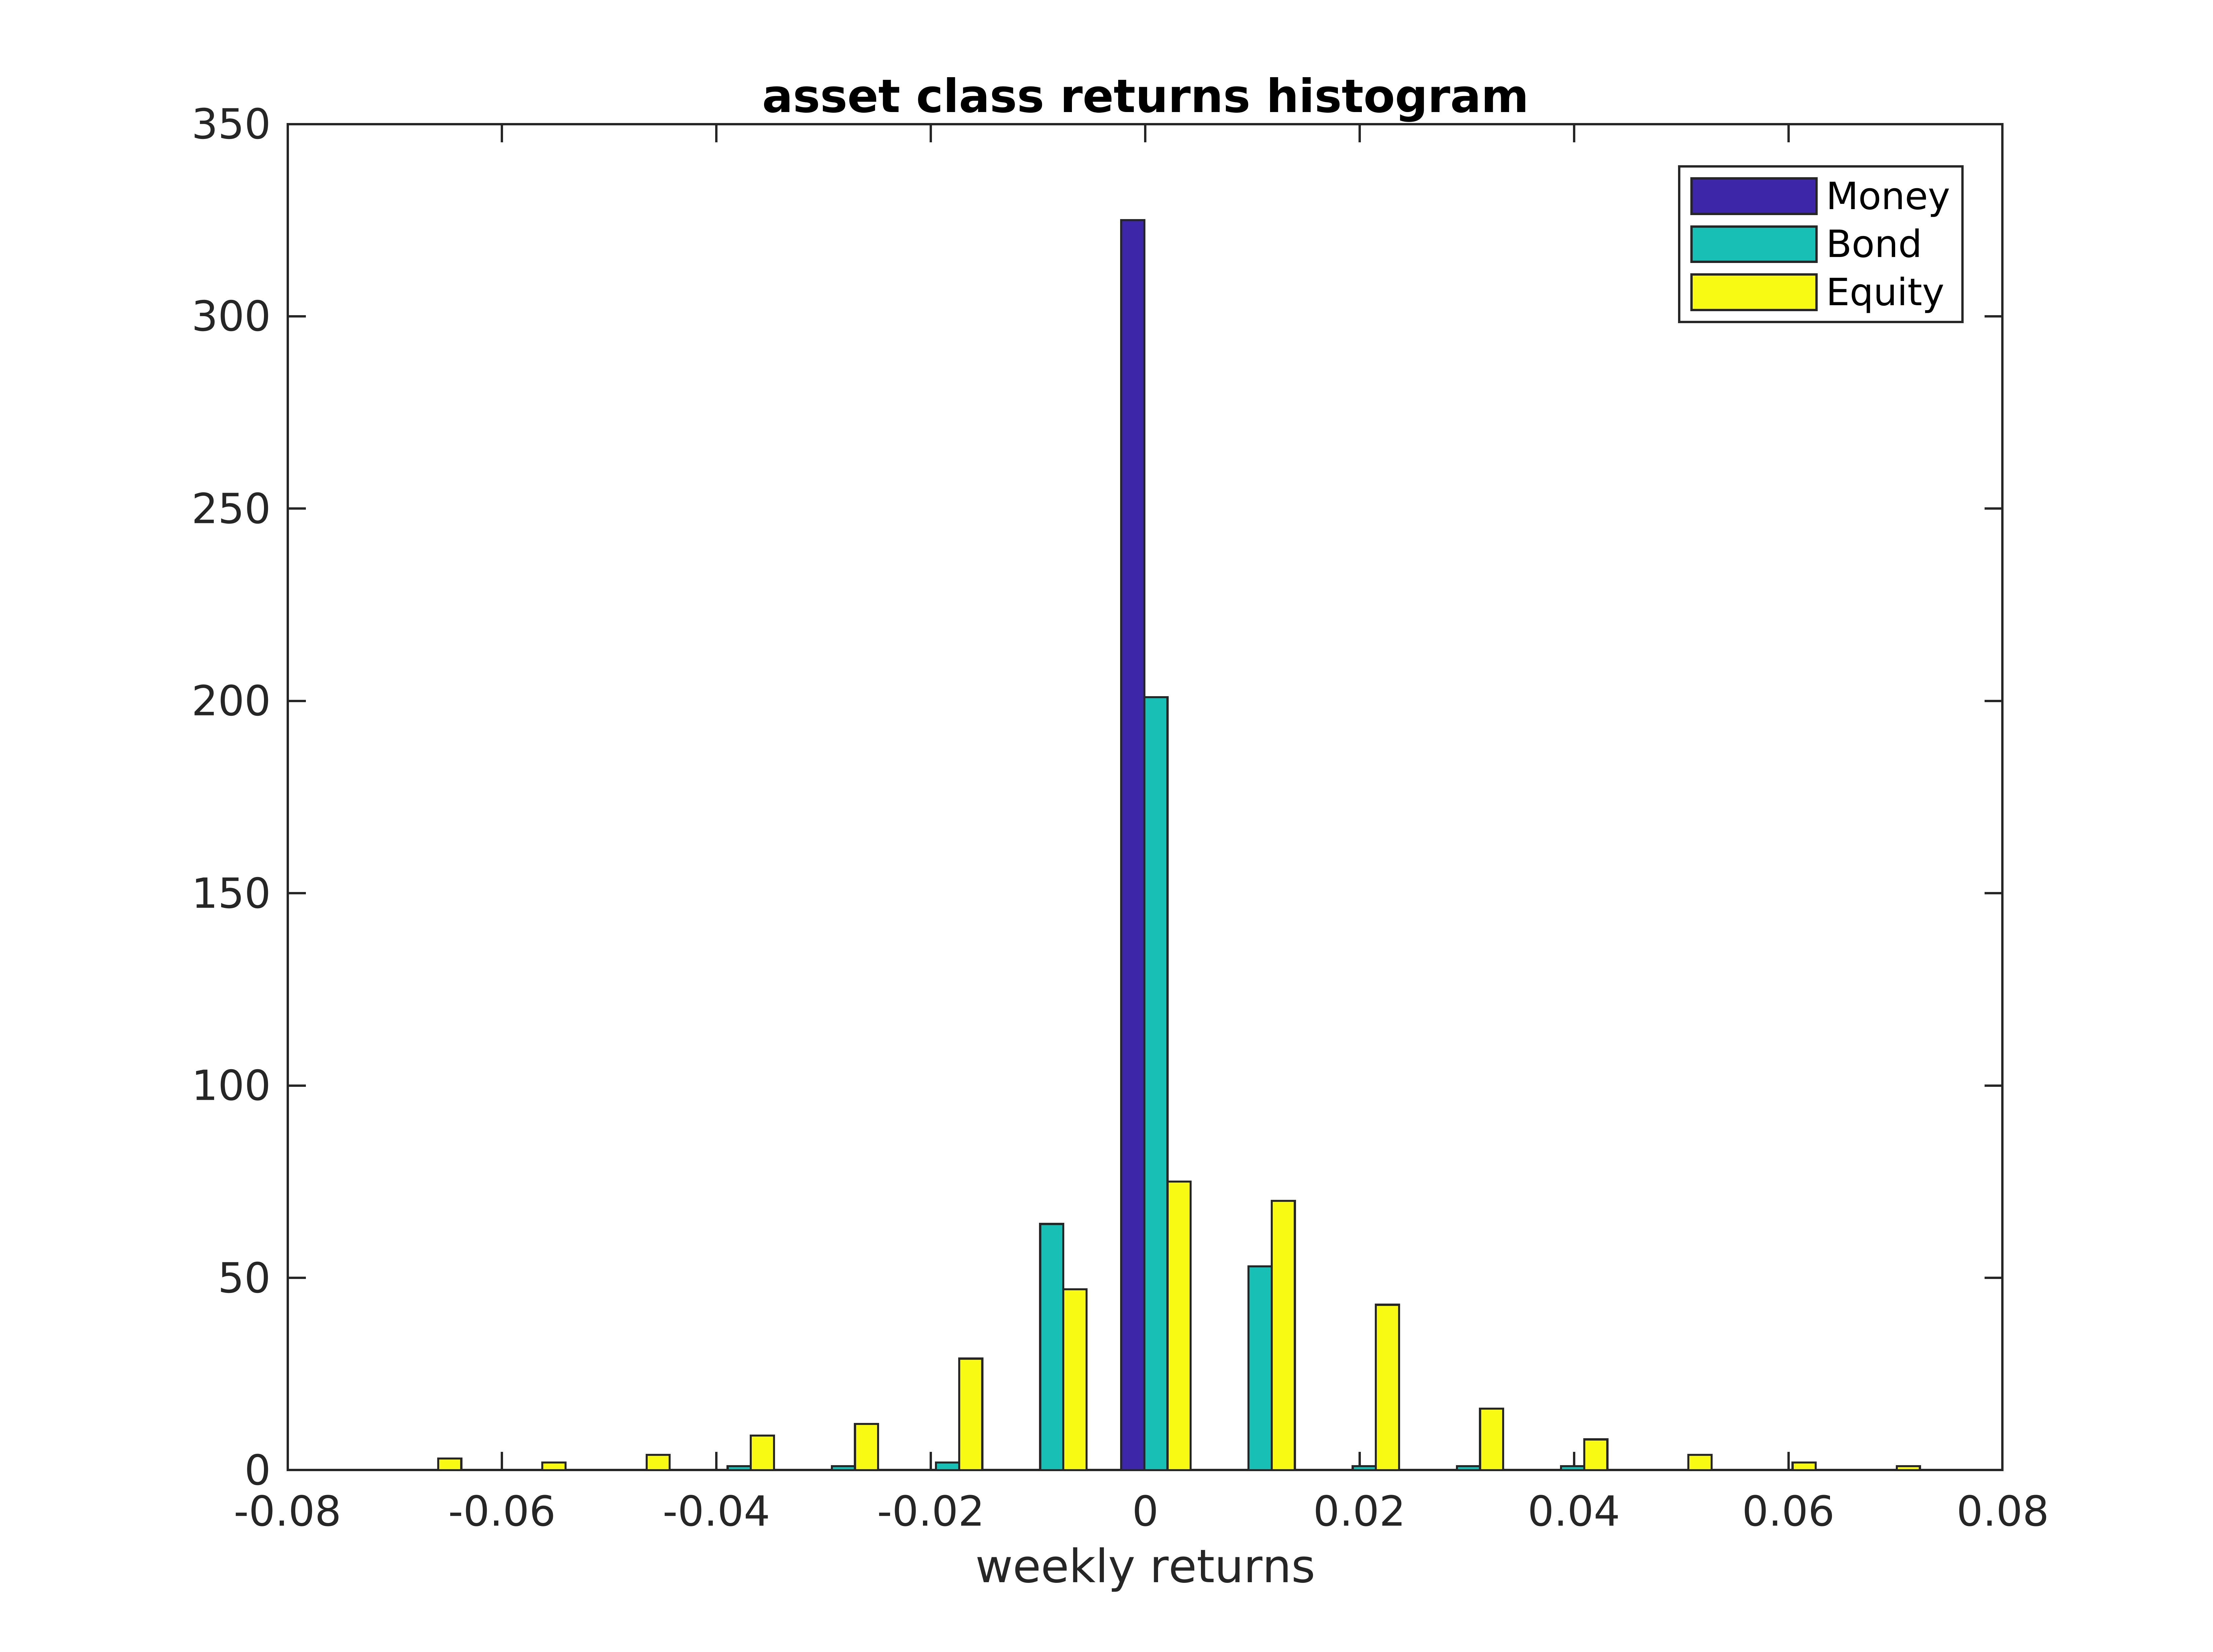
\includegraphics[scale=0.6]{Images/ReturnsHist.png}
	\caption{Weekly asset class returns histogram.}
\end{figure}
\begin{table}[H]\label{tab:sampleStatistics}
	\centering
	\begin{tabular}{@{}llll@{}} \toprule
		Statistic & C & B & E \\ \midrule
		Mean Return (ann) & 0.064\%  & 3.46\% & 12.11\%\\
		\addlinespace[0.5em]
		Volatility (ann) & 0.113\%  & 4.81\% & 14.81\% \\
		\addlinespace[0.5em]
		Median (ann) &	0\% & 4.58\% & 17.74\% \\
		\addlinespace[0.5em]
		Skewnwss & 0.262 & -0.0621 & -0.36 \\
		\addlinespace[0.5em]
		Kurtosis & 3.90 & 10.62 & 4.42 \\
		\addlinespace[0.5em]
		Monthly $V@R_{0.95}$ & 0.0808\% & 3.73\% & 14.95\%\\
		\addlinespace[0.5em]
		Max Drawdown & 0.106\% & 5.87\% & 23.98\% \\
		\addlinespace[0.5em]
		Mean Drawdown & 0.020\% & 1.5\% & 4.62\% \\
		\addlinespace[0.5em]
		Sharpe ratio & 0 & 0.692 & 0.767 \\ \bottomrule
		\addlinespace[0.5em]
	\end{tabular}
	\caption{Asset class returns sample statistics}
\end{table}

Finally, the sample correlation matrix is  
\[ 
\begin{bmatrix}
1 & 0.166 & -0.075 \\
  &  1    & -0.454 \\
  &       &  1
\end{bmatrix}.
\]

\section{Optimal Allocation Maps}\label{sec:Allocation_Maps}
Let us consider an asset allocation problem characterized by the following parameters:
\begin{itemize}
	\item 2-year investment horizon
	\item weekly rebalancing frequency, which means $N=104$ portfolio rebalancings
	\item monthly value-at-risk equals to 7\%
	\item target return $\theta=7\%$ per year
	\item initial wealth $x_0 = 1$
\end{itemize}
The target sets we want our portfolio value to stay within are 
\begin{align*}
X_0 & = \{1\}\\
X_k & = [0,\infty) \quad k = 1,\ldots,103 \\
X_{104} & = [(1+\theta)^2,\infty) = [1.07^2,\infty)
\end{align*}
In practice, these sets are discretized with a discretization step of $10^{-3}$ and truncated where the probability measure is negligible; the actual sets used in the implementation thus are $X_k = [0.5,1.9]$ $k=1,\ldots,103$, $X_{104}=[(1.07)^2,1.9]$. As stated in Problem \ref{prb:ODAA}, we are looking for a sequence of allocation maps which maximize the following joint probability
\[ \mathbb{P}\big(\{\omega \in \Omega : x_0 \in X_0,\ldots,x_{104} \in X_N \} \big).\]
The final choice to be made before running the algorithm is picking a model for the asset class returns. As a first example, we opt for the GM model which has been fitted to data applying the Expectation-Maximization method (see Subsection \ref{subsec:EM}) which brings the following results:
\begin{align*}
\bm{\mu}_1 & = 
\begin{bmatrix}
\num{1.385e-5} &  \num{1.023e-3} &  \num{2.327e-3}
\end{bmatrix}
\quad & \bm{\Sigma}_1 &= 
\begin{bmatrix}
\num{2.567e-8} & \num{8.011e-8} & \num{-2.090e-7} \\
& \num{2.330e-5}  & \num{-6.263e-5} \\
&                & \num{4.453e-4}
\end{bmatrix} \\
\bm{\mu}_2 & = \begin{bmatrix}
\num{1.638e-6} &  \num{-2.088e-3} &  \num{1.255e-3}
\end{bmatrix}
\quad & \bm{\Sigma}_2 &= 
\begin{bmatrix}
\num{1.760e-8} & \num{8.430e-7} & \num{-4.984e-7} \\
& \num{1.937e-4}  & \num{-6.250e-5} \\
&                & \num{2.395e-4}
\end{bmatrix}
\end{align*}
and $\lambda = 0.881$.
By applying the backward algorithm enunciated in Theorem \ref{thm:rec_algo}, we obtained the maps reported in Figure \ref{fig:mapsMixture}
\begin{figure}[h]\label{fig:mapsMixture}
	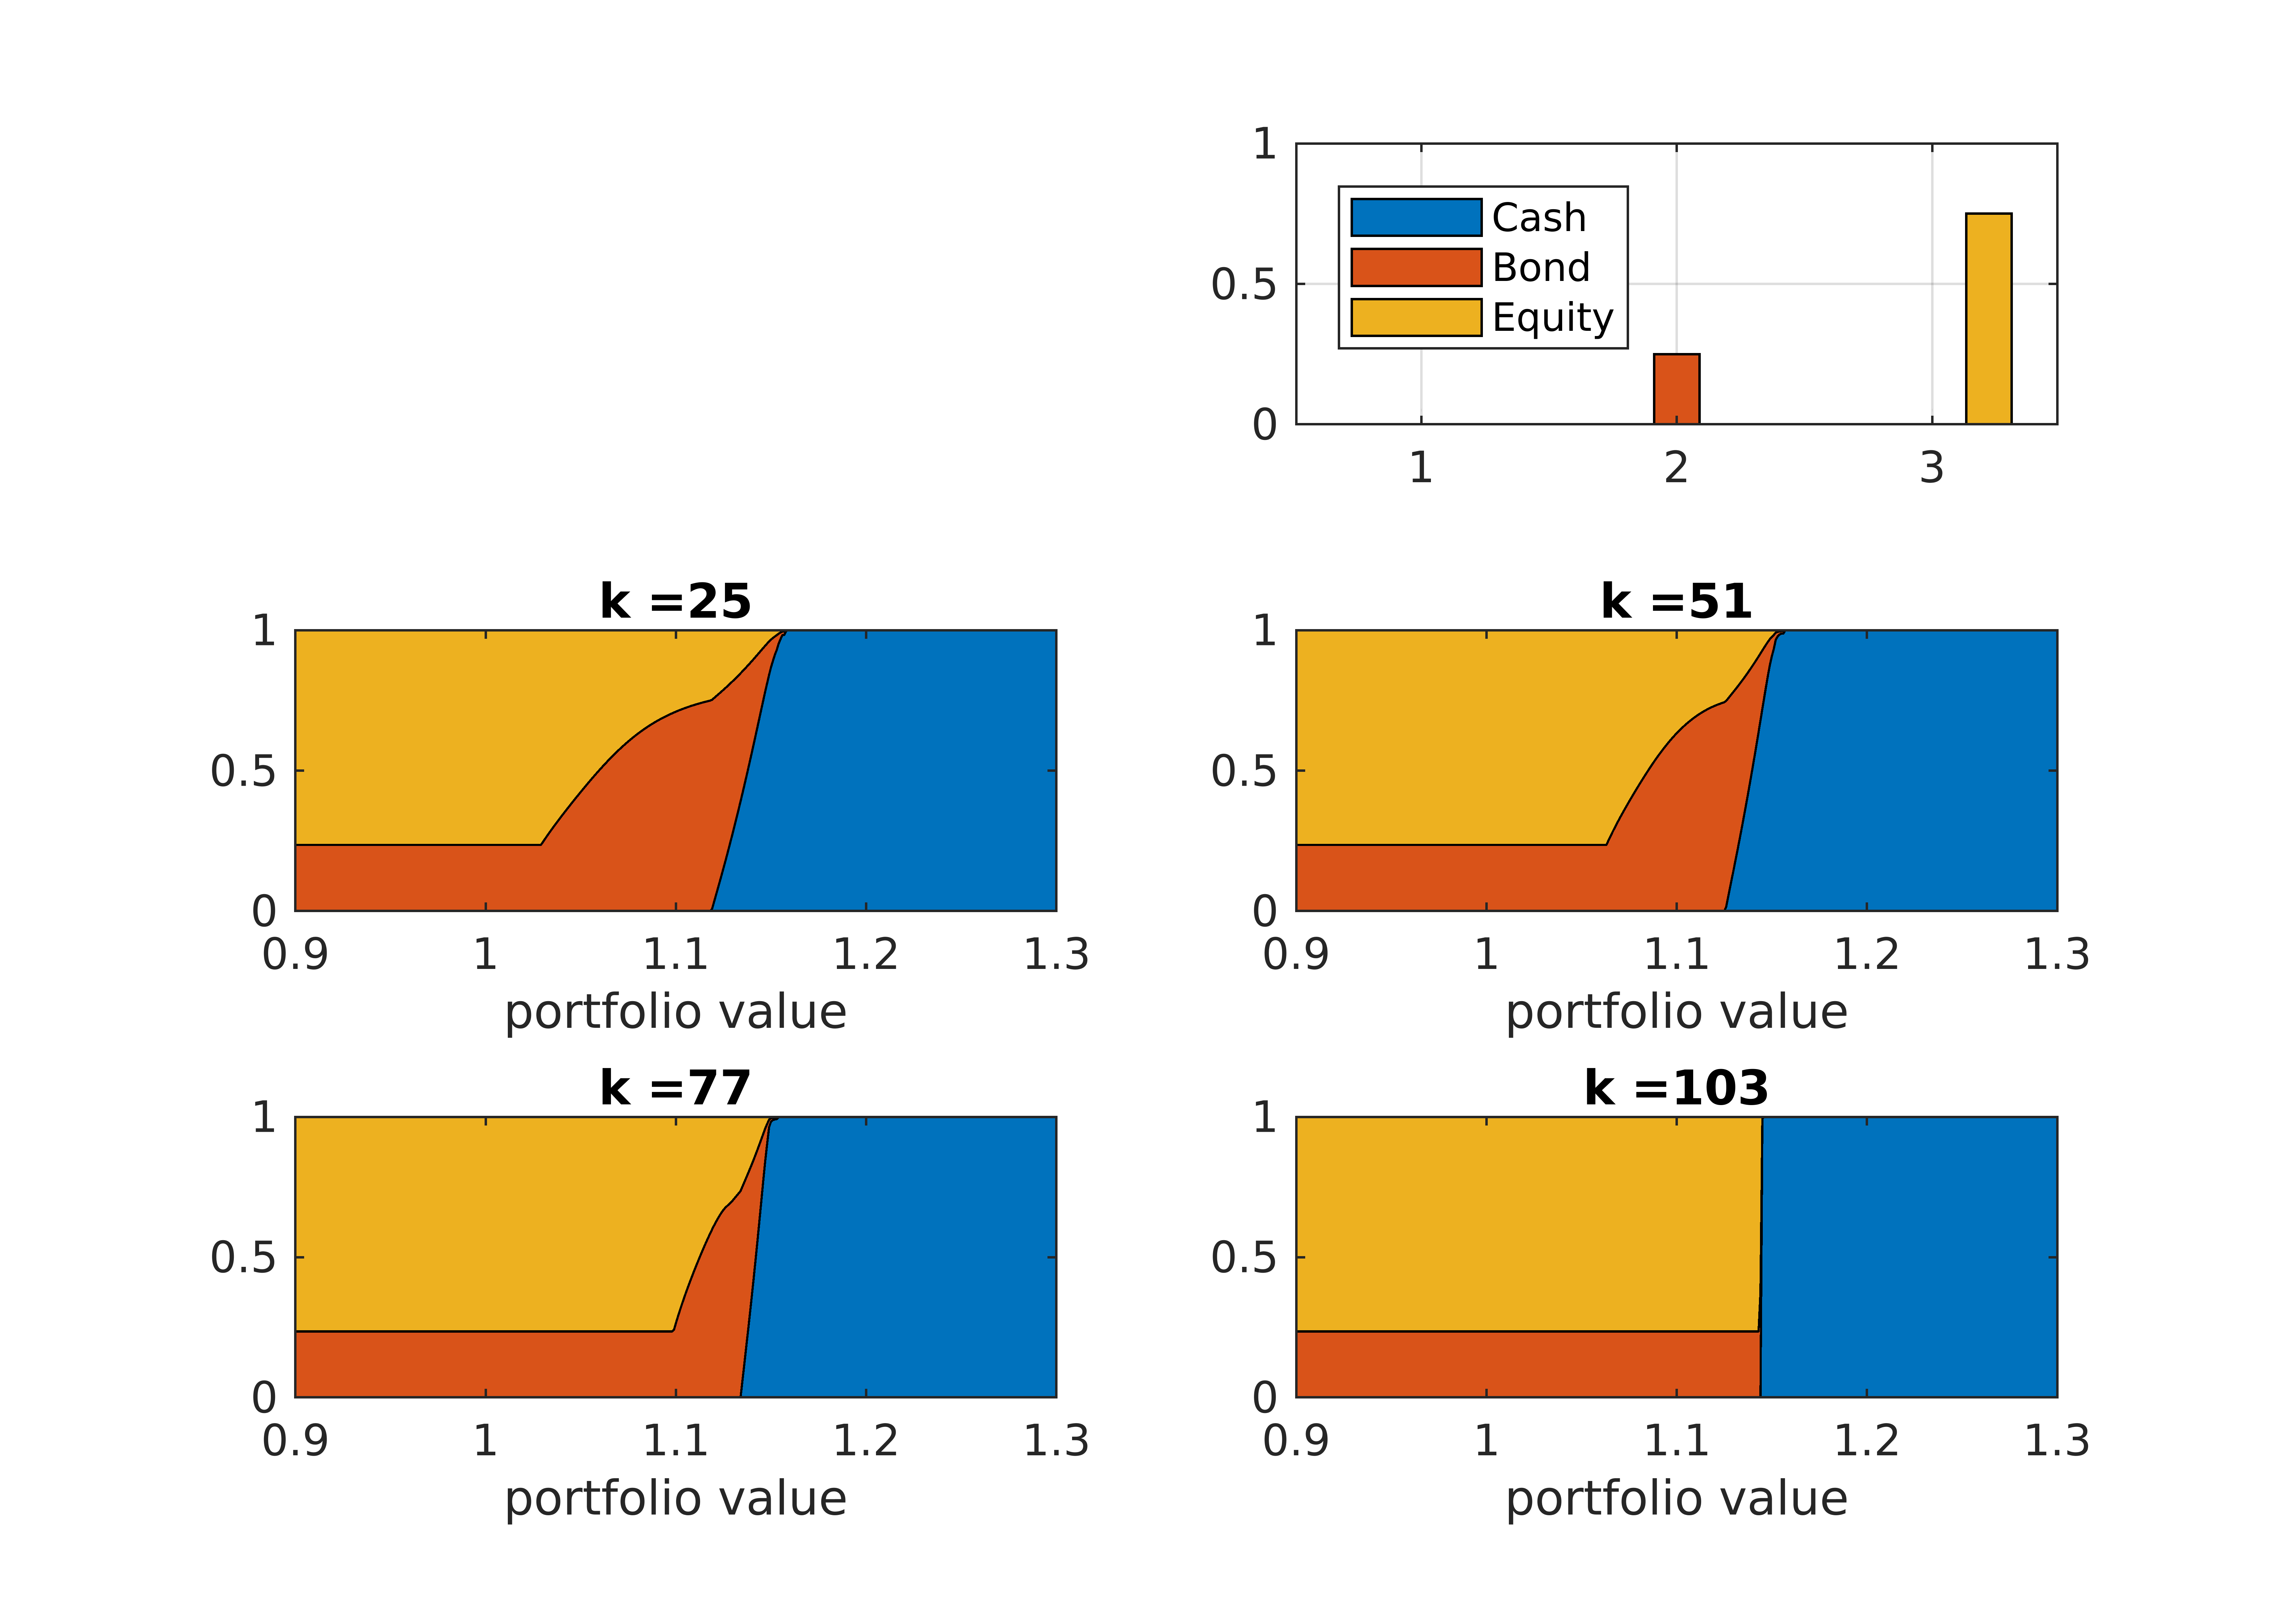
\includegraphics[scale = 0.9]{Images/mapsMixturewk.png}
	\caption{Optimal allocation maps, weekly rebalancing, GM model}
\end{figure}


Let us now take the time to analyze the kind of investment strategy these maps imply. At the beginning of the investment ($k=0$), the optimal strategy prescribes that 25.34\% of investor's wealth be invested in Bond and 74.66\% in Equity. After 25 weeks, depending on the realization of portfolio value (x-axis in Figure \ref{fig:mapsMixture}), the optimal strategy tells us to allocate wealth as follows: if the portfolio is underperforming (its value is in the \textit{danger} zone, approximately below \$1.028), the optimal allocation is a mix of Equity and Bond, that is the riskiest mix allowed (a 100\% allocation in Equity is not allowed due to the \text{risk} constraint). As soon as performance gets better (the \textit{neutral} zone is from \$1.028 to \$1.16) the Equity weight decreases in favor of more Bond and from a certain point on also Cash. When the portfolio is outperforming (the \textit{safe} zone is above \$ 1.16), the whole wealth is invested in Cash, the least risky of the three asset classes. This kind of investing strategy is known in the literature with the name of \textit{contrarian} strategy. The name stems from the fact that contrarian investors bet against the prevailing market trend, namely they try to sell "high" and buy "low". Contrarian strategies perform well is volatile markets and poorly in trending market due to their convex nature. The optimal strategy obtained by the ODAA algorithm exhibits the same pattern also at successive rebalancing times, the only difference is that it becomes more extreme while approaching the end of the investment; for instance, at time $k=103$ there is no transition from the riskiest allocation to the least risky one (if the target has not been reached before the last week, the strategy will do whatever it takes to get there by assuming the riskiest exposure).

\begin{table}[h]
	%\renewcommand{\arraystretch}{0.5}
	\centering
	\resizebox{\textwidth}{!}{\begin{tabular}{@{}*{10}{c}@{}}
		\toprule
		& \multicolumn{3}{c}{G} & \multicolumn{3}{c}{GM} & \multicolumn{3}{c}{NIG} \\
		\addlinespace[0.5em]
		\cmidrule(l){2-4} \cmidrule(l){5-7} \cmidrule(l){8-10} 
		& wk & m & q 	& wk & m & q 	& wk & m & q\\
		\addlinespace[0.5em]
	$p^{\star}$ & 79.67\% & 75.56\% & 73.26\% & 78.72\%  & 73.35\% & 69.52\% & 78.53\% & 73.24\% &69.47\%  \\
	\addlinespace[0.5em]
	$p_{MC}$ & 79.77\% & 75.56\% & 73.28\% & 78.73\%  & 73.40\% & 69.49\% & 78.76\% & 73.30\% &69.32\%  \\
	\addlinespace[0.5em]	
	time[h] & 0.698 & 0.157 & 0.050 & 0.904  & 0.357 & 0.234 & 6.131 & 1.467 &0.371  \\	\bottomrule
	\end{tabular}}
	\caption{Probability of reaching the target set obtained via  ODAA algorithm ($p^{\star}$) and Monte-Carlo simulation ($p_{MC}$) for the Gaussian (GM), Gaussian Mixture (GM) and Normal Inverse Gaussian (NIG) model. Time is the computation time of the ODAA algorithm in hours.}
\end{table}

\begin{table}[]
	
	\centering
	\begin{tabular}{@{}*{4}{c}@{}}
		\toprule
	Moment	& G & GM & NIG \\
		\addlinespace[0.5em]
		\midrule	
	$\mu_{x_{k+1}}$	& & & \\
	\addlinespace[0.5em]	
	$\sigma_{x_{k+1}}$	& & & \\
	\addlinespace[0.5em]
	$\gamma_{x_{k+1}}$	& & & \\
	\addlinespace[0.5em]
	$\kappa_{x_{k+1}}$	& & & \\
	\addlinespace[0.5em]
	\bottomrule
	\end{tabular}
\end{table}
